\section{Introduction}
We will analyse the research paper we read and the hardware and software components used.
\section{Related Literature Review}
T. Perković et al., surveyed on this parking system and they took behaviour on some sensors. They used ultrasound sensor, IR sensor, photo diode and magnetometer. They took the output signal of those sensors on car parked and on no parked state. They plotted those output signals data and compare among those sensor. They used cloud server to store data and used computer to visualize slot status \cite{PERKOVIC2020121181}. M. Prasanth et al., Proposed a system on this topic based on internet of things technology. They used Raspberry pi, IR obstacle sensor and RFID for verification. They send parking slot status to user using wifi module. They did not use any cloud server to store data or any security system \cite{prasanth12design}.
Attiqur et al., devepoloped a system where they used RFID, Raspberry pi and ultrasonic sensor. They used wifi module to send data to local mysql server. Their system has not any security feature or location system \cite{atiqursmart}. 
Koushika et al., developed a system in which they used image processing technology to identify the slot status. They collected image from CCTV and processed it using raspberry pi. They did the image processing steps like image detection, edge detetion etc. After processing image they send the slot status to remote server and using mobile application user can interact with the system. \cite{koushika2021efficient}
DivyanshuShekhar et al., proposed a system on online parking system. They made web app, the owner can post the slot status with this application and user can see the free slot area of this parking space. This system is not automated \cite{divyanshushekhar2021parkofy}. 
N. R. Siva Jyothi et al., developed their system on smart parking. They used sensor, raspberry pi, cloud server, user application and operator application. Sensors take the slot status and send to server using raspberry pi. User can entrance and exit using \cite{jyothireal}
Attiqur et al., developed a system where they Used ultrasonic sensor, raspberry pi, Wifi and RFID. They developed ios application to book the parking slot \cite{atiqur2020automated}. 
D.Azshwanth et al., developed a system on smart parking. They used CMOS, ultrasonic and Electro-magnetic sensor for checking the apearance of car in parking slot. With arduino and modem they transmit slot status to the receiver. They built up payment system using mobile application. Their application has no anti theft feature \cite{azshwanth2019automated}.
Mrs. D.J. Bonde et al., developed a system where interfaced LCD with microcontroller, interfaced GSM with microcontroller, interfacing RF module with microcontroller and developed and android application. Sensor data are sent to parking system using RF and then this status was sent to android using GSM module \cite{bonde2014automated}. 
Natarajan et al., developed car parking system where they used IR sensor for reading the status when cars enter and exit the place. They used RIO to send signals to lab view. for every slot they used led. for free and parked condition they used LEDs of different color \cite{natarajan2018design}.
Mohammed Azher Therib et al., developed a system where they used counter. When a car is entered the counter increased by one and when leave counter decreased by one. when the count is same to slot number the gate turned off by a servo motor. When count is less than slot number gate is automatically turned on \cite{doi}. 
Samir A. El-Seoud et al., developeed a system which can read car plate automatically and stores the car information in a dynamic database. Web application and android application can retrieve those data and can pay fare solution electronically \cite{el2016towards}.
\cite{fernando2020innovation}
Inhwan Jung et al., developed a system on smart parking. In their system they used arduino, ethernet shield and ultrasonic sensor. With ultrasonic sensor they detect the appearance of car. With ethernet shield they transferred data to database. With smartphone application they visualized status and could interact with the system \cite{international2018managment}.
% \cite{lou2020iot}
P.Raghava Reddy et al., developed a smart parking system based on IoT technology. Servo motor, blynk application, RFID and ESP8266 module was used for this system. Everything was computed by arduino and sent to database using NodeMCU.\cite{khanna2016iot}
% \cite{shimi2020intelligent}
Putri Sandika Juwita et al., developed a system in which they used ultrasonic sensor for every slot and a NodeMCU. Sensor can detect appearance of car and with NodeMCU signals can send to central raspberry pi. Raspberry pi acquired all of those data and send the slot status to firebase database. Using web application those status could retrieve \cite{juwita2020smart}.

\section{Hardware Specification}
\subsection{Arduino Mega 2560}
The Arduino Mega 2560 is an ATmega2560-based microcontroller board. There are 54 digital pins for input and output (of which 14 can be used as PWM outputs). It includes everything which need to support the microcontroller. A usb cable is needed to link it to computer or power it to start. The arduino is suitable for most Arduino Duemilanove and Diecimila shields.
\begin{figure}[H]
\centering
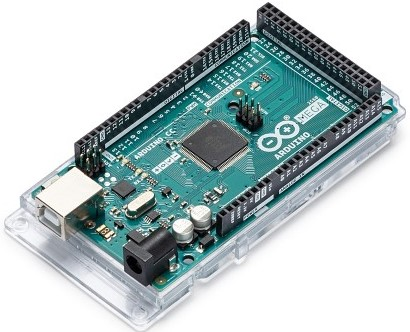
\includegraphics[width=0.5\textwidth]{figures/Arduino Mega.jpg}
\caption{Arduino Mega.}
\label{Arduino Mega}
\end{figure}
\subsection{GSM Module}
A GSM (Global System for Mobile Communications) module is a device that is used to send data to a remote network via mobile GSM technology. It can transport a data rate of 64 kbps up to 120 Mbps.
\begin{figure}[H]
\centering
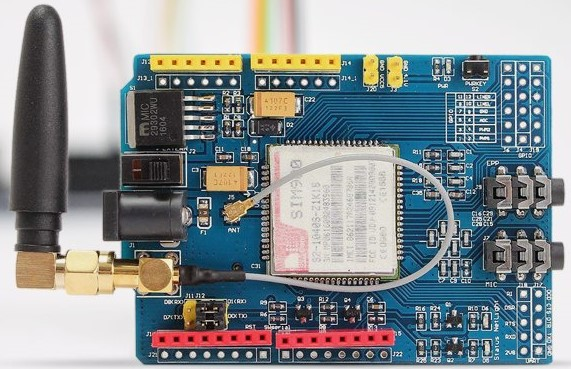
\includegraphics[width=0.5\textwidth]{figures/GSM Shield with Arduino.jpg}
\caption{GSM Module.}
\label{GSM module}
\end{figure}
\subsection{16*2 LCD Display}
LCD refers to the word liquid crystal display. LCD display is very commonly used in most embedded projects, the reason being its cheap price, availability and programmer friendly. 
\begin{figure}[H]
\centering
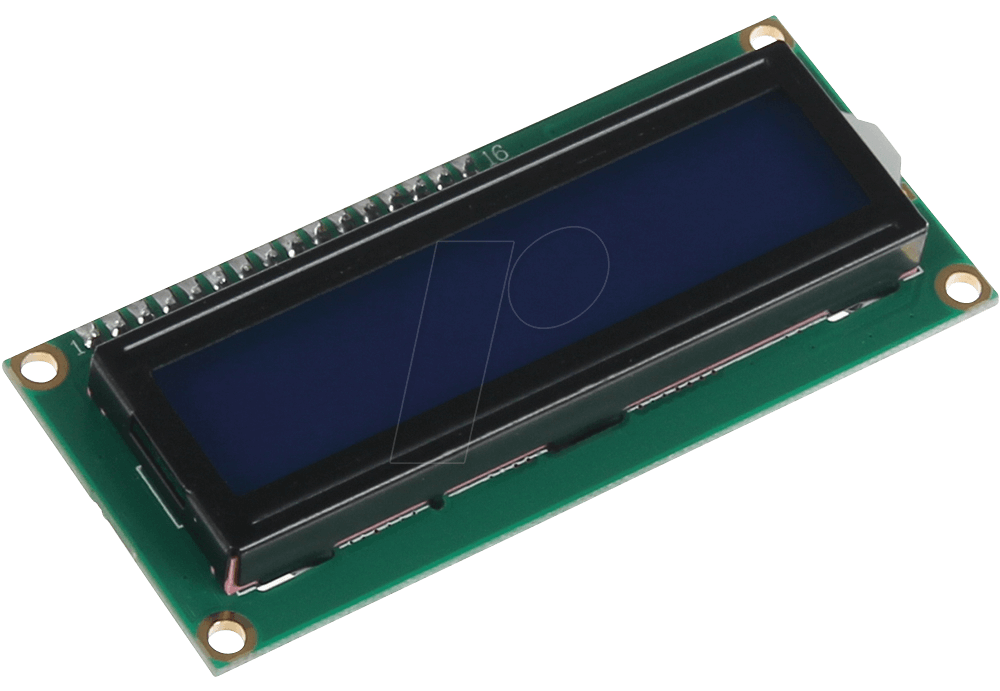
\includegraphics[width=0.5\textwidth]{figures/16x2 LCD.png}
\caption{16*2 LCD Display.}
\label{LCD Display}
\end{figure}
\subsection{4*4 Keypad}
The 4*4 matrix keypad usually used as input in a project. It contains a total of 16 keys, meaning the same input values. Every column and row keys are attached by external pins.
\begin{figure}[H]
\centering
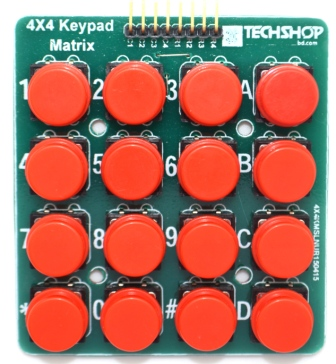
\includegraphics[width=0.5\textwidth]{figures/Keypad.jpg}
\caption{4*4 Keypad.}
\label{Keypad}
\end{figure}
\subsection{IR Obstacle Sensor}
The infrared (IR) obstacle sensor has a pair of infrared transmitting and receiving sensors. The infrared LED emits Infrared signals at certain frequency and when an obstacle appears on the line of infrared light, it is reflected back by the obstacle which is sensed by the receiver. When an impediment is detected by the sensor the LED indicator is illuminated and a signal is given via the OUT pin. The sensor contains a potentiometer that is adjustable for changing the sensor distance.
\begin{figure}[H]
\centering
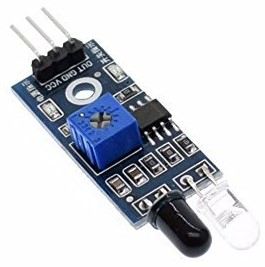
\includegraphics[width=0.5\textwidth]{figures/irinfrared-obstaclR-avoidance-sensor.jpg}
\caption{IR Obstacle Sensor.}
\label{IR obstacle sensor}
\end{figure}
\subsection{Buzzer}
The buzzer is a sound system that converts electricity signals to sound signals. It is usually powered by DC voltage. It is commonly utilized as sound devices in alarms, computers, printers and other electronic equipments. The buzzer may generate sounds like music, siren, buzzer, alarm and electric bell.
\begin{figure}[H]
\centering
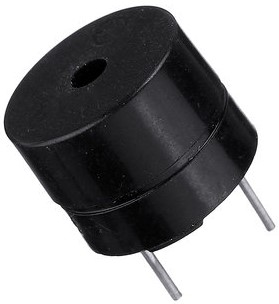
\includegraphics[width=0.5\textwidth]{figures/Buzzer.jpg}
\caption{Buzzer.}
\label{Buzzer}
\end{figure}
\subsection{Servo Motor}
A servo engine is a small, lightweight high-performance shaft unit. Servo can rotate approximately 180 degrees (90 in each direction) and works just like the standard kinds. To manage these servos, anybody can utilize servo code, hardware or library. Mainly in computers, toys, CD/DVD players, the servo motor is used.
\begin{figure}[H]
\centering
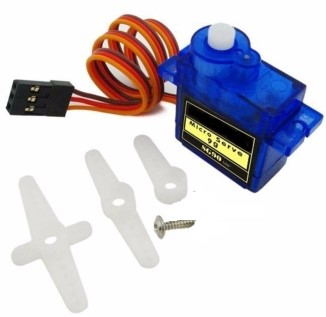
\includegraphics[width=0.5\textwidth]{figures/Servo Motor.jpg}
\caption{Servo Motor.}
\label{Servo motor}
\end{figure}
\subsection{NodeMCU ESP8266}
NodeMCU ESP8266 is a cheap WiFi device including a complete TCP/IP stack and a microprocessor.It has a library to transmit and retrieve data to a remote server.It is very easy to use and to combine with another arduino.
\begin{figure}[H]
\centering
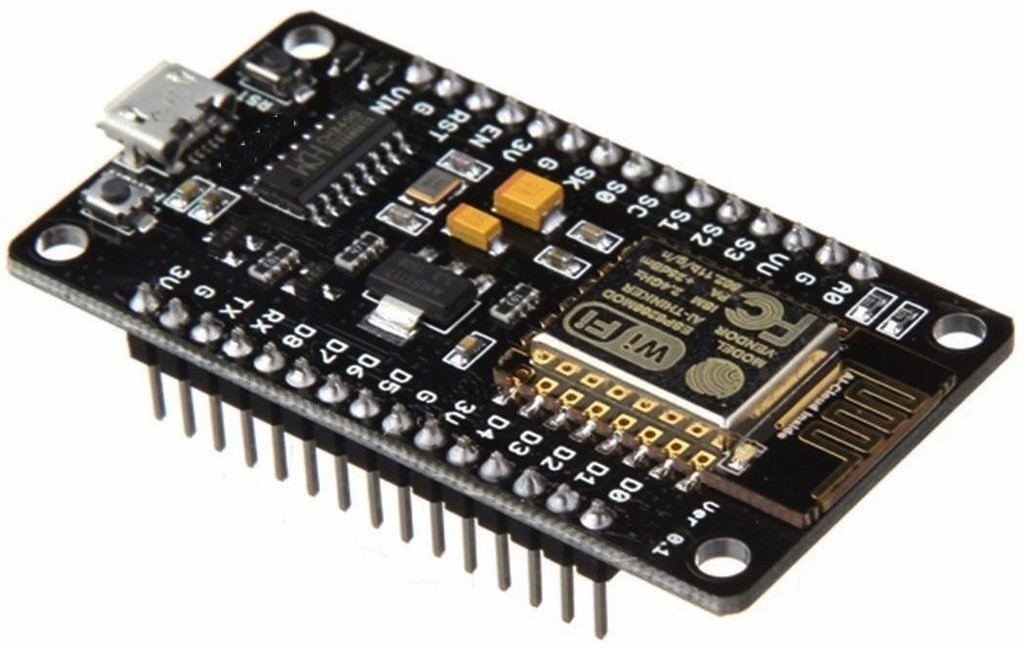
\includegraphics[width=0.5\textwidth]{figures/NodeMCU_ESP8266_development_board_1024x1024.jpg}
\caption{NodeMCU.}
\label{NodeMCU}
\end{figure}
\subsection{Other Equipments}
Other passive equipments like a breadboard, jumper wire, adapter, scotch tape, gum and plywood is used. A breadboard is a solderless device for temporary prototype with electronics and test circuit designs. Jumper wire is an electrical wire which is normally used to interconnect the components of a breadboard or other prototype or test circuit.
\begin{figure}[H]
\centering
\subfloat[Breadboard]{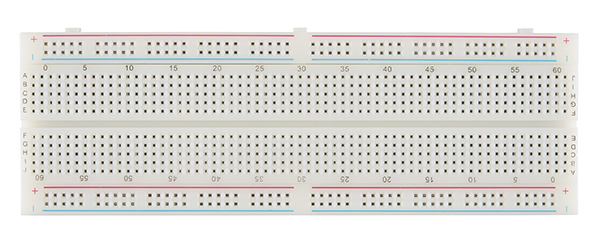
\includegraphics[width = 0.3\textwidth]{figures/Breadboard.jpg}} 
\hspace{1cm}
\subfloat[Jumper wire]{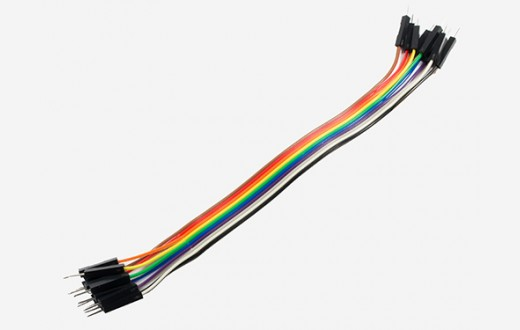
\includegraphics[width = 0.3\textwidth]{figures/Jumper Wire.jpg}}
\hspace{1cm}
\subfloat[Plywood]{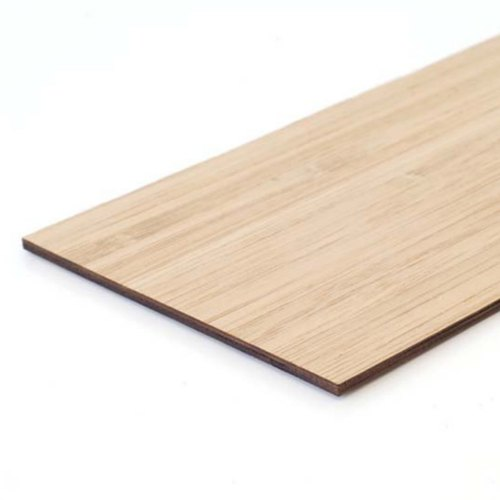
\includegraphics[width = 0.3\textwidth]{figures/Plywood.jpg}} 
\hspace{1cm}
\subfloat[Adapter]{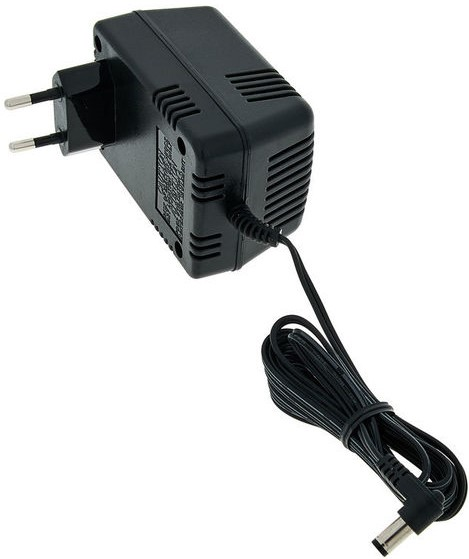
\includegraphics[width = 0.2\textwidth]{figures/Adapter.jpg}}
\hspace{1cm}
\caption{Other components}
\label{Other1}
\end{figure}
\section{Software Specification}
\subsection{Arduino IDE}
This platform is used to write Arduino board code. It is a C language based IDE. The Arduino board has its own compiler and library loaded. The Arduino board is used for IDE editing, debugging and loading. It features a serial monitor that allows us to observe any real-time value. Learning and using it is really simple.
\begin{figure}[H]
\centering

\includegraphics[width=0.5\textwidth]{figures/Arduino Software.png}
\caption{Arduino.}
\label{Arduino IDE}
\end{figure}
\subsection{Android Studio}
Android Studio is made by IntelliJ for writing code for android device. It is an IDE for java and a broad XML language. It has got his own android device compiler. For a different version of the android operating system, some libraries have already been installed. Code can be modified, dubbed and exported to APK applications using this platform.
\begin{figure}[H]
\centering
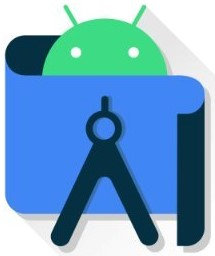
\includegraphics[width=0.5\textwidth]{figures/Android Studio.jpg}
\caption{Android Studio.}
\label{Android Studio}
\end{figure}
\subsection{Firebase}
We used the realtime firebase database as our database's cloud server. This platform is made by Google. It is faster, easy and free to use. It features SDK and an Arduino code API so it's easy to integrate.
\begin{figure}[H]
\centering
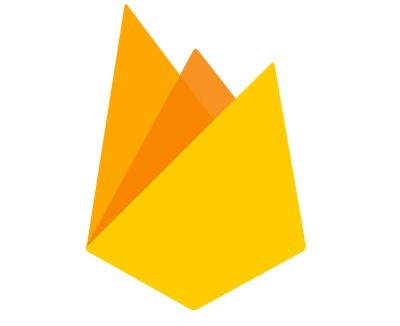
\includegraphics[width=0.5\textwidth]{figures/Firebase real.jpg}
\caption{Firebase.}
\label{Firebase}
\end{figure}
\subsection{Web Browser}
A web browser is an application used to access and view websites. If a user requires a web page from a certain web site, a web browser will retrieve the required content of a web server and display the page on the device of the user. The main purpose of a web browser is to return HTML, the code for designing or "fixing" online pages.
\begin{figure}[H]
\centering
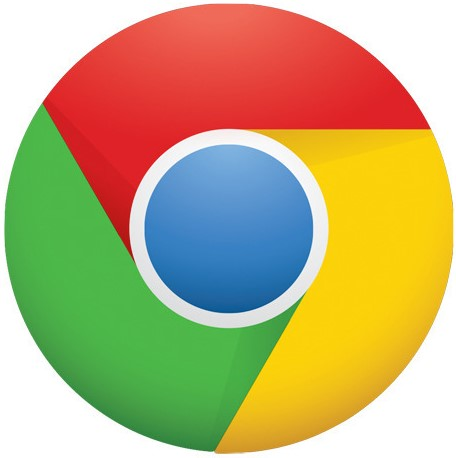
\includegraphics[width=0.4\textwidth]{figures/Web Browser.jpg}
\caption{Web Browser.}
\label{Web Browser}
\end{figure}
\subsection{Implementation Challenges}
\begin{itemize}
    \item To make the system durable
    \item To make the system simple
    \item To store data securely 
    \item Connectivity and Power measurement
    \item Continuous internet and power supply challenge
    \item To manage all the component of good quality
\end{itemize}


\section{Conclusion}
In this chapter we discussed the previous work on smart parking system. We analysed and found limitation of their works. We discussed on hardware and software we have used in this project. In the following chapter we will provide vast explanation on smart car parking system.